\documentclass[12pt,a4paper]{article}

% Margins.
\setlength{\oddsidemargin}{0in}
\setlength{\evensidemargin}{0in}
\setlength{\headheight}{12pt}
\setlength{\headsep}{42pt}
\setlength{\topmargin}{-54pt}
\setlength{\textwidth}{6.5in}
\setlength{\textheight}{10in}

\usepackage{amsmath}
\usepackage{float}
\usepackage{graphicx}
\usepackage[hyphens]{url}
\usepackage{hyperref}	% Clickable links to figures, references and urls.
\usepackage{enumerate}

% Drawing.
\usepackage{pgf}
\usepackage{tikz}

% Listings for formatting code.
\usepackage{listings}
\usepackage{textcomp}
% General options.
\lstset{breaklines=true, basicstyle=\small\ttfamily, tabsize=4, numbers=left, stepnumber=1, frame=single, showstringspaces=false, upquote=true}
% C++ specific high-lighting. Comments are 50/50 shades of green/black and strings coloured with 60/40 red/black mixture.
\lstset{language=[ISO]C++, commentstyle=\color{green!50!black}, keywordstyle=\color{blue}, stringstyle=\color{red!60!black}}

%opening
\title{\vspace{-2cm}Programming for Engineers II\\Class 27\\Passing Pointer to Pointer in Function\\Linked List Concept}
\author{Attique Dawood}
\date{April 03, 2013\\[0.2cm] Last Modified: \today}
\begin{document}
\maketitle
\section{Announcements}
\begin{itemize}
\item None.
\end{itemize}
\section{Revision}
\begin{itemize}
\item \texttt{this} pointer.
\item \texttt{void} pointer.
\item \texttt(const) pointer.
\end{itemize}
\section{\texttt{sizeof() struct or class}}
\begin{itemize}
\item If there is only one data member then size of object is the size of data member. For example size of \verb|class X { char t; }| object is 1 byte.
\item For default settings, if there are more than 1 members then size is a multiple of `struct package size'. Default package size is 8 bytes.
\item A class with one char and one double is 9 bytes, so with default package size object will be of 16 bytes in memory.
\end{itemize}
\begin{figure}[H]
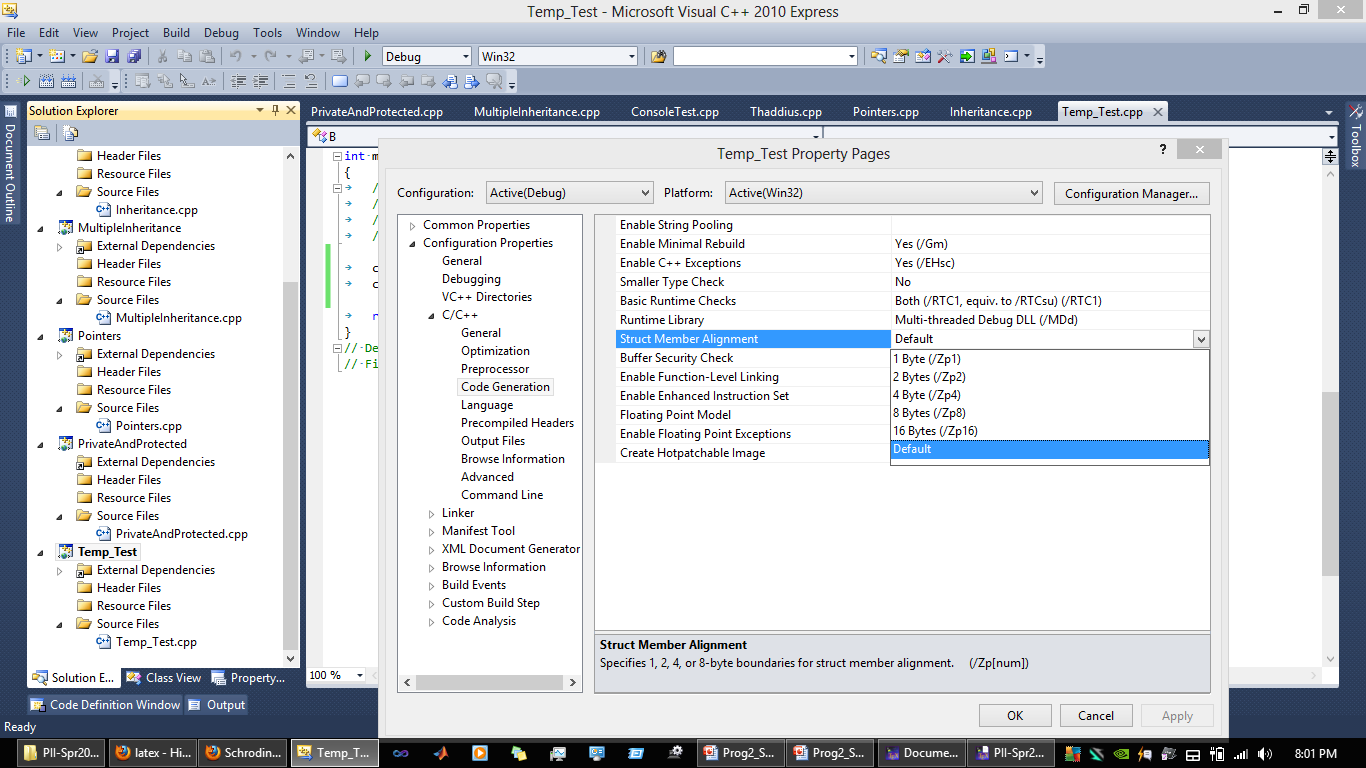
\includegraphics[width=\textwidth]{StructPackagingSize}
\end{figure}
\section{Constant String}
\begin{lstlisting}[caption={constant string}]
#include <iostream>
using namespace std;

int main()
{
	char str1[] = "Defined as an array";
	char* str2 = "Defined as a pointer";
	cout << str1 << endl; // display both strings
	cout << str2 << endl;
	//str1++; //can’t do this; str1 is a const ptr
	str2++; // this is OK, str2 is a pointer
	cout << str2 << endl; //now str2 starts "efined..."

	return 0;
}
\end{lstlisting}
\begin{lstlisting}[caption={Array of constant strings, contiguous storage}]
#include <iostream>
using namespace std;

int main()
{
	const int DAYS = 7;
	char* arrptrs[DAYS] = { "Sunday", "Monday", "Tuesday", "Wednesday", "Thursday", "Friday", "Saturday" };

	for(int j=0; j<DAYS; j++) //cout every string
		cout << arrptrs[j] << endl;

	return 0;
}
\end{lstlisting}
\begin{lstlisting}[caption={Constant column length, non-contiguous storage},escapechar=!]
#include <iostream>
using namespace std;

int main()
{
	const int DAYS = 7;
	!\color{red}{char arrptrs[DAYS][10]}! = { "Sunday", "Monday", "Tuesday", "Wednesday", "Thursday", "Friday", "Saturday" };

	for(int j=0; j<DAYS; j++) //cout every string
		cout << arrptrs[j] << endl;

	return 0;
}
\end{lstlisting}
\section{Argc and Argv}
\begin{itemize}
\item When running a program from commandline, you can pass arguments to main.
\item First argument is always the name of the program.
\item Argc is count of arguments including program name and argv is a char** to argument strings.
\end{itemize}
\begin{lstlisting}[caption={Passing Arguments to main()}]
#include <iostream>
#include <string>
using namespace std;

int main(int argc, char** argv)
{
	cout << "Number of arguments = " << argc << endl;
	cout << "Argument list: " << endl;
	for (int i=0; i<argc; i++)
		cout << "Arg " << i+1 << " = " << argv[i] << endl;

	string pass = "password";
	if (pass == string(argv[1]))
		cout << "Correct Password!" << endl;
	else
		cout << "Incorrect Password." << endl;

	return 0;
}
\end{lstlisting}
\section{Passing Pointers to Function}
\begin{itemize}
\item How can we change value of a variable in function? Two solutions: pass as reference, or pass as pointer.
\item How can we return two values of different type? Pass variables as reference or pointers.
\item To change int, we pass \textcolor{red}{pointer--to--int} or \verb|int*| in the function.
\item If we want to change a pointer, we'll need to pass \textcolor{red}{pointer--to--pointer} or \verb|int**|.
\end{itemize}
\begin{lstlisting}[caption={Passing Variable as Reference and as Pointer}]
#include <iostream>
using namespace std;

void SquareRef(int& x)
{
	x = x*x;
}
void SquarePtr(int* x)
{
	*x = *x * *x;
}
int main()
{
	int a = 3;
	int b = 5;

	SquareRef(a);
	SquarePtr(&b);

	cout << "a^2 = " << a << endl;
	cout << "b^2 = " << b << endl;

	return 0;
}
\end{lstlisting}
\begin{lstlisting}[caption={Function that `returns' int and double}]
#include <iostream>
using namespace std;

void Square(int* x, double* y)
{
	*x = *x * *x;
	*y = *y * *y;
}
int main()
{
	int a = 3;
	double b = 5;

	Square(&a, &b);

	cout << "a^2 = " << a << endl;
	cout << "b^2 = " << b << endl;

	return 0;
}
\end{lstlisting}
\begin{lstlisting}[caption={Function to Allocate Array}]
#include <iostream>
using namespace std;

void CreateArray(int** ArrayPtr, int* SizePtr)
{
	cin >> *SizePtr;
	*ArrayPtr = new int[*SizePtr];
}
int main()
{
	int* Array;
	int Size;

	CreateArray(&Array, &Size);

	return 0;
}
\end{lstlisting}
\section{Linked List}
\begin{itemize}
\item Storage problems with fragmented memory or hard disk.
\item Array requires contiguous space in memory. Array cannot dynamically grow incrementally. Must de--allocate and re--allocate whole array to change size.
\item Linked list solves the above problems. Doesn't require contiguous memory. Linked list is a chain of pointer--connected nodes. Nodes store information just like array indices.
\item Linked list access is slower than array. Must traverse whole list to reach a particular node. But, storage and size is flexible.
\item Array is preferable when speed is desired and storage size is known. Static data. Example: Number of students in a class cannot exceed 50. An array of 50 size for students is most appropriate in this scenario.
\item Linked list is preferable when speed is not a major concern and storage size is highly dynamic. Example: Daily record of cars using motorway. On weekends traffic is high but there aren't many cars on weekdays. Number of cars can be highly varied. Linked list is most suited for storing daily information of each car.
\end{itemize}
%\nocite{*}
%\bibliographystyle{plain}
%\bibliography{OOPref}
\end{document}
